\documentclass{article}

\usepackage[section]{incertia}

\pagestyle{fancy}
\lhead{Will Song}
\chead{Representation Theory of $\sl(2, \CC)$}
\rhead{\today}

\begin{document}
\textbf{Disclaimer:} The vast majority of this essentially comes from Pavel
Etingof's \textit{Introduction to Representation Theory} chapter 2.

\section{Introduction}
Before we actually talk about the representation theory of $\sl(2, \CC)$, we
first need to talk about the basics.

\begin{df}
An \textbf{associative algebra} $A$ is a vector space that is equipped with an
associative bilinear operator $\cdot : A \times A \to A$. We are only interested
in the associative algebras with multiplicative unit.
\end{df}

\begin{ex}
The \textbf{endomorphism ring} $\End(V)$ of a vector space $V$ can be made into
an associative algebra with function composition. The elements of $\End(V)$ are
linear operators $T : V \to V$ and the identity is $\id_V(v) = v$.
\end{ex}

\begin{df}
A \textbf{homomorphism of algebras} $\varphi : A \to B$ is a linear map that
preserves the algebra structure. e.g. $\varphi(xy) = \varphi(x) \varphi(y)$.
\end{df}

\begin{df}
A \textbf{representation} of an algebra $A$ is a vector space $V$ together with
a homomorphism of algebras $\rho : A \to \End(V)$.

You can think of this as giving $A$ an action (or a left module structure) on
$V$. We will interchange the notation $\rho(a, v) = \rho(a)(v) = a \cdot_{\rho}
v = a \cdot \rho = av$ very often.
\end{df}

\begin{df}
A \textbf{subrepresentation} of a representation $V$ is a subspace $W \subseteq
V$ such that $W$ is invariant under the operators of $A$. In other words,
$\set{aw : a \in A, w \in W} \subseteq W$.
\end{df}

\begin{df}
A representation $V$ is said to be \textbf{irreducible} if the only
subrepresentations are $0$ and $V$.
\end{df}

\begin{prop}
If $V$ and $W$ are representations of an algebra $A$, then $V \oplus W$ has an
obvious structure as a representation of $A$.
\end{prop}

\begin{proof}
$a (v, w) = (av, aw)$.
\end{proof}

\begin{df}
A representation is said to be \textbf{indecomposable} if it cannot be written
as the direct sum of two non-zero representations.
\end{df}

\begin{df}
A \textbf{homomorphism of representations} or \textbf{intertwining operator}
between two representations $V, W$ of the associative algebra $A$ is a linear
map $\varphi : V \to W$ that commutes with the action of $A$. e.g. $\varphi(av)
= a \varphi(v)$.

A homomorphism of representations is an \textbf{isomorphism of representations}
if it is an isomorphism of vector spaces.
\end{df}

\begin{prop}[Schur's Lemma]
Let $V, W$ be representations of an associative algebra $A$ over a field (not
necessarily algebraically closed) $K$ and let $\phi : V \to W$ be a non-zero
homomorphism of representations. Then
\begin{enumerate}
\item
$V$ irreducible implies $\phi$ is injective.
\item
$W$ irreducible implies $\phi$ is surjective.
\end{enumerate}
\end{prop}

\begin{proof}
$ $
\begin{enumerate}
\item
$\ker \phi$ is a subrepresentation of $V$. $V$ is irreducible so it must be
either $0$ or $V$. Since $\phi$ is non-zero it must be $0$.
\item
$\phi(V)$ is a subrepresentation of $W$. A similar argument applies.
\end{enumerate}
\end{proof}

\begin{cor}
Let $V$ be a finite dimensional irreducible representation of an algebra $A$
over an algebraically closed field $K$. Let $\phi : V \to V$ be a non-zero
homomorphpism of representations. Then $\phi = \lambda \id$, for some $\lambda
\in K$.
\end{cor}

\begin{proof}
$\phi$ has an eigenvalue $\lambda \in K$ because $K$ is algebraically closed.
Verify that $\phi - \lambda \id$ is a homomorphism of representations which is
not an isomorphism (it has determinant $0$). By Schur's Lemma, it must be the
zero map which implies the result.
\end{proof}

\begin{df}
A \textbf{Lie algebra} $\mathfrak{g}$ is a vector space over a field $K$ with a
skew-symmetric bilinear map $[-,-] : \mathfrak{g} \times \mathfrak{g} \to
\mathfrak{g}$, e.g. $[a, a] = 0$, satisfying the \textbf{Jacobi identity}
\[ [[a, b], c] + [[b, c], a] + [[c, a], b] = 0. \]
\end{df}

\begin{ex}
Any associative algebra can be made into a Lie algebra by using the commutator
bracket $[a, b] = ab - ba$.
\end{ex}

\begin{ex}
The special linear Lie algebra of order $n$ over $\CC$ $\sl(n, \CC)$ is the
space of $n \times n$ matrices with trace $0$ under the commutator bracket. For
example, $\sl(2, \CC)$ has basis
\[ e = \begin{pmatrix} 0 & 1 \\ 0 & 0 \\ \end{pmatrix} \qquad f =
\begin{pmatrix} 0 & 0 \\ 1 & 0 \\ \end{pmatrix} \qquad h = \begin{pmatrix} 1 & 0
\\ 0 & -1 \\ \end{pmatrix}. \]
This has relations $[e, f] = h$, $[e, h] = -2e$, and $[f, h] = 2f$.
\end{ex}

\begin{df}
A \textbf{homomorphism of Lie algebras} $\varphi : \mathfrak{g}_1 \to
\mathfrak{g}_2$ is a linear map that preserves the Lie bracket. e.g.
$\varphi([a, b]) = [\varphi(a), \varphi(b)]$.
\end{df}

\begin{df}
A \textbf{representation} of a Lie algebra $\mathfrak{g}$ is a vector space $V$
with a homomorphism of Lie algebras $\rho : \mathfrak{g} \to \End(V)$, where
$\End(V)$ is a Lie algebra due to the commutator bracket.
\end{df}

\begin{df}
The \textbf{universal enveloping algebra} $\mathcal{U}(\mathfrak{g})$ of a Lie
algebra $\mathfrak{g}$ is the free algebra on $\mathfrak{g}$ modulo the
relations $xy - yx = [x, y]$.
\end{df}

\begin{rem}
One can show that a representation of $\mathfrak{g}$ is essentially the same as
a represeentation of $\mathcal{U}(\mathfrak{g})$ and vice versa. This makes
talking about representations of Lie algebras a lot easier because we know a lot
more about the representation of algebras.
\end{rem}

\begin{rem}
We also have a Schur lemma for Lie algebras, but due to representations of Lie
algebras being the same as representations of their universal enveloping
algebras, we can just use the normal Schur lemma.
\end{rem}

\newpage
\section{Representation Theory}
Recall that a representation of $\sl(2)$ is just a vector space $V$ with three
operators $E$, $F$, and $H$, such that $HE - EH = 2E$, $HF - FH = -2F$, and $EF
- FE = H$, where the corresponding map $\rho$ is given by $\rho(e) = E, \rho(f)
= F, \rho(h) = H$, where $e, f, h$ are defined as they were previously.

Let $V$ be a finite dimensional representation of $\sl(2, \CC)$.

\begin{prop}
Take eigenvalues of $H$ and pick one with the biggest real part. Call it
$\lambda$. Let $\bar{V}(\lambda)$ be the generalized eigenspace of $\lambda$.
Show that $E|_{\bar{V}(\lambda)} = 0$.
\end{prop}

\begin{proof}
Let $v$ be any element from $\bar{V}(\lambda)$. We show that $Ev = 0$. Namely,
$v$ satisfies $(H - \lambda \id)^k v = 0$, for some integer $k$. We will examine
$E(H - \lambda \id)^k v = 0$. In particular, I claim $E(H - \lambda)^k = (H - (2
+ \lambda))^k E$. For the case $k = 1$, we can see that $E(H - \lambda) = HE -
2E - \lambda E = (H - 2 - \lambda) E$. For the inductive step, $E(H - \lambda)^k
(H - \lambda) = (H - (2 + \lambda))^k E (H - \lambda) = (H - (2 + \lambda))^k (H
- (2 + \lambda)) E$, so indeed $E(H - \lambda)^k = (H - (2 + \lambda))^k E$. We
can now get
\[ 0 = E(H - \lambda \id)^k v = (H - (2 + \lambda) \id)^k (Ev) = 0. \]
Thus either $Ev$ is $0$ or $Ev$ is a generalized $(\lambda + 2)$-eigenvector of
$H$, but the real part of $\lambda + 2$ if larger than the real part of
$\lambda$, which contradicts maximality so $Ev = 0$.
\end{proof}

\begin{prop}
Let $W$ be any representation of $\sl(2, \CC)$ and let $w \in W$ be a non-zero
vector such that $Ew = 0$. For any $k > 0$, find a polynomial $P_k(x)$ of degree
$k$ such that $E^k F^k w = P_k(H) w$.
\end{prop}

\begin{proof}
\begin{lem}
We have the commutator relations
\[ \begin{aligned}
[H, E^k] &= 2k E^k, \\
[H, F^k] &= -2k F^k, \\
[E, F^k] &= k H F^{k - 1} + k(k - 1) F^{k - 1}. \\
\end{aligned} \]
\end{lem}
\begin{proof}[Solution]
We only show the inductive steps, because the base cases are trivial. For $[H,
E^k]$, compute
\[ \begin{aligned}
H E^k - E^k H  &= H E^k - E (E^{k - 1} H) \\
&= H E^k - E (H E^{k - 1} - 2(k - 1) E^{k - 1}) \\
&= H E^k - (E H) E^{k - 1} + 2(k - 1) E^k \\
&= H E^k - (H E - 2 E) E^{k - 1} + 2(k - 1) E^k \\
&= H E^k - H E^k + 2 E^k + 2(k - 1) E^k \\
&= 2k E^k. \\
\end{aligned} \]
The proof for $[H, F^k]$ follows from exactly the same procedure. For $[E,
F^k]$, compute
\[ \begin{aligned}
E F^k - F^k E &= E F^k - F (F^{k - 1} E) \\
&= E F^k - F (E F^{k - 1} - (k - 1) H F^{k - 2} - (k - 1)(k - 2) F^{k - 2}) \\
&= E F^k - (F E) F^{k - 1} + (k - 1)(F H) F^{k - 2} + (k^2 - 3k + 2) F^{k - 1}
\\
&= E F^k - (E F - H) F^{k - 1} + (k - 1)(H F + 2F) F^{k - 2} + (k^2 - 3k + 2)
F^{k - 1} \\
&= H F^{k - 1} + (k - 1) H F^{k - 1} + (2k - 2) F^{k - 1} + (k^2 - 3k + 2) F^{k
- 1} \\
&= k H F^{k - 1} + (k^2 - k) F^{k - 1}, \\
\end{aligned} \]
as desired.
\end{proof}

We first compute $E F^k w = (k H F^{k - 1} + k(k - 1) F^{k - 1}) w$. We can now
apply $E^{k - 1}$ to both sides to obtain
\[ \begin{aligned}
E^k F^k w &= (k E^{k - 1} H F^{k - 1} + k(k - 1) F^{k - 1}) w \\
&= (k (H E^{k - 1} - 2(k - 1) E^{k - 1}) F^{k - 1} + k(k - 1) E^{k - 1} F^{k -
1}) w \\
&= (k H - 2k(k - 1) + k(k - 1)) E^{k - 1} F^{k - 1} w \\
&= k (H - (k - 1)) E^{k - 1} F^{k - 1} w, \\
\end{aligned} \]
or $P_k(H) = k(H - (k - 1)) P_{k - 1}(H)$, with $P_1(H) = H$. Now one can easily
show that
\[ P_k(H) = k! H (H - 1) \cdots (H - (k - 1)), \]
where $P_k(H)$ is obviously a polynomial of degree $k$ in $H$.
\end{proof}

\begin{prop}
Let $v \in \bar{V}(\lambda)$ be a generalized eigenvector of $H$ with eigenvalue
$\lambda$. Show that there exists $N > 0$ such that $F^n v = 0$.
\end{prop}

\begin{proof}
We claim $F(H - \lambda)^k = (H - (\lambda - 2))^k F$. For the induction step,
compute
\[ \begin{aligned}
F(H - \lambda)^k (H - \lambda) &= (H - (\lambda - 2))^k F (H - \lambda) \\
&= (H - (\lambda - 2))^k (H - (\lambda - 2)) F, \\
\end{aligned} \]
as desired. Because $v \in \bar{V}(\lambda)$ of $H$, we have $(H - \lambda
\id)^k v = 0$ for some integer $k$. We apply $F$ to both sides, to obtain $(H -
(\lambda - 2) \id)^k (Fv) = 0$, or $Fv$ is a $\lambda - 2$ generalized
eigenvector of $H$ whenever $v$ is a $\lambda$ generalized eigenvector of $H$.
Because $\bar{V}(\lambda)$ is finite dimensional ($V$ is finite dimensional),
there can only be finitely many eigenvalues (and thus non-zero generalized
eigenspaces), but the maximal chain of eigenvalues is $\dim V$ long, so we can
say $F^{\dim V} v = 0$.
\end{proof}

\begin{prop}
Show that $H$ is diagonalizable on $\bar{V}(\lambda)$.
\end{prop}

\begin{proof}
To show that $E$ is diagonalizable on $\bar{V}(\lambda)$, we show that every
vector $v \in \bar{V}(\lambda)$ is an ordinary eigenvector.

\begin{lem}
If $v$ is a generalized eigenvector of $H$ with eigenvalue $\lambda$, and $a_1,
\dots, a_n \in \CC$ such that
\[ (H - a_1) \cdots (H - a_n) v = 0, \]
then there exists some $i$ such that $a_i = \lambda$.
\end{lem}

\begin{proof}
We proceed via induction on $n$.  If $n = 1$, then the statement $(H - a_1)v =
0$ just means that $Hv = a_1v$, or $a_1 = \lambda$ from our assumption. If $n >
1$, then either $(H - a_n)v = 0$, implying $a_n = \lambda$ or $(H - a_1) \cdots
(H - a_{n - 1})((H - a_n)v) = 0$, where $(H - a_n)v$ is a generalized
eigenvector with eigenvalue $\lambda$, so we are done by our induction
hypothesis.
\end{proof}

We can use the formula deduced in problem 2 (because $E$ is zero on
$\bar{V}(\lambda)$) to compute
\[ E^N F^N v = k! H (H - 1) \cdots (H - (N - 1)) v = 0, \]
where $N$ is chosen such that $F^N v = 0$ for $v \in \bar{V}(\lambda)$. We now
know that $\lambda \in \set{0, \dots, N - 1}$. Notice that the $(H - i)$ all
commute with each other, so we can write
\[ k! \left( \prod_{i \neq \lambda} (H - i) \right) ((H - \lambda)v) = 0. \]
If $(H - \lambda)v$ is a non-zero generalized eigenvector with respect to
$\lambda$, then one of the $i$'s must be equal to $\lambda$, which is clearly
untrue, so $(H - \lambda)v = 0$, or $v$ is a standard eigenvector with
eigenvalue $\lambda$ on $H$. Since this holds for all $v$, it is clear that $H$
is diagonalizable.
\end{proof}

\begin{prop}
Let $N_v$ be the smallest $N$ satisfying (c). Show that $\lambda = N_v - 1$.
\end{prop}

\begin{proof}
Take $N_v$ as defined and notice that $v, Fv, \dots, F^{N_v - 1} v$ are all
non-zero by definition. By problem 5, $v$ must be an ordinary eigenvector of
$H$.

Recall that $EF^k v = kHF^{k - 1} v + k(k - 1) F^{k - 1} v$ and $HF^k - F^k H =
-2k F^k$, or $HF^k = F^k H - 2kF^k$, so
\[ \begin{aligned}
EF^k v &= k (F^{k - 1} H - 2 (k - 1) F^{k - 1}) v + k (k - 1) F^{k - 1} v \\
&= k (F^{k - 1} H v - (k - 1) F^{k - 1} v) \\
&= k (\lambda F^{k - 1} v - (k - 1) F^{k - 1} v) \\
&= k (\lambda - k + 1) F^{k - 1} v. \\
\end{aligned} \]
We can also compute $HF^k v = F^k H v - 2k F^k v = (\lambda - 2k) F^k v$, so $v,
Fv, \dots, F^{N_v - 1} v$ are all ordinary eigenvectors of $H$.

It now becomes clear that $E^k F^k v = \alpha_k v$ for some $\alpha_k \neq 0$.
Thus, $E^{N_v - 1} F^{N_v - 1} v \neq 0$. From the equation $E^{N_v} F^{N_v} v =
0$, we see that $\lambda \in \set{0, \dots, N_v - 1}$. However, if $\lambda \in
\set{0, \dots, N_v - 2}$, then $E^{N_v - 1} F^{N_v - 1} v = 0$, which is clearly
not the case, so we necessarily have $N_v = \lambda + 1$.
\end{proof}

\begin{rem}
Let $V(\lambda)$ denote the ordinary eigenspace of $H$ corresponding to
$\lambda$. Then we have the following sort of diagram
\begin{center}
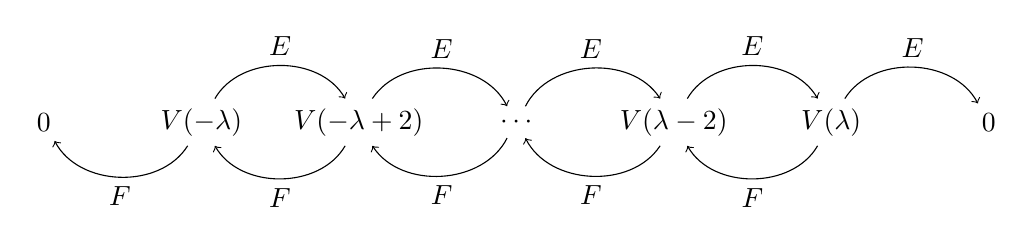
\begin{tikzpicture}
\node (la)  at (6, 0)  {$0$};
\node (la0) at (4, 0)  {$V(\lambda)$};
\node (la2) at (2, 0)  {$V(\lambda - 2)$};
\node (ccc) at (0, 0)  {$\cdots$};
\node (lb2) at (-2, 0) {$V(-\lambda + 2)$};
\node (lb0) at (-4, 0) {$V(-\lambda)$};
\node (lb)  at (-6, 0) {$0$};

\path[->]
(la0) edge[bend left=60] node[below] {$F$} (la2)
(la2) edge[bend left=60] node[below] {$F$} (ccc)
(ccc) edge[bend left=60] node[below] {$F$} (lb2)
(lb2) edge[bend left=60] node[below] {$F$} (lb0)
(lb0) edge[bend left=60] node[below] {$F$} (lb)
(lb0) edge[bend left=60] node[above] {$E$} (lb2)
(lb2) edge[bend left=60] node[above] {$E$} (ccc)
(ccc) edge[bend left=60] node[above] {$E$} (la2)
(la2) edge[bend left=60] node[above] {$E$} (la0)
(la0) edge[bend left=60] node[above] {$E$} (la)
;
\end{tikzpicture}
\end{center}
where $H$ acts as a scalar on each subspace.
\end{rem}

\begin{prop}
Show that for each $N > 0$, there exists a unique up to isomorphism irreducible
representation of $\sl(2)$ of dimension $N$. Compute the matrices $E, F, H$ in
this representation using a convenient basis.
\end{prop}

\begin{proof}
Let $V$ be a finite-dimensional irreducible representation of $\sl(2, \CC)$ of
dimension $N$. We fix an eigenvalue with maximal real part $\lambda$ and we fix
a vector $v \in \bar{V}(\lambda)$ of $H$. We claim that the vectors $v, Fv,
\dots, F^{\lambda} v$ form a basis for $V$.

We know that $F^{\lambda + 1} v = 0$ from problem 5, so $v, Fv, \dots,
F^{\lambda} v$ are all non-zero eigenvectors of $H$ with eigenvalues $\lambda,
\lambda - 2, \dots, -\lambda$, respectively, which implies their linear
independence. Once we show that these vectors span $V$, then we can establish
the relationship $N = \lambda + 1$.

Recall that a subrepresentation is invariant under the operators of its parent
representation. Applying $E$, $F$, and $H$ do not introduce any elements outside
of the span, by the computations from problem 5, so the span of these vectors is
clearly a subrepresentation and because $V$ is irreducible, it must be $V$.

The action of $H$ on $V$ is represented with the diagonal matrix consisting of
$\lambda, \lambda - 2, \dots, -\lambda$ on the main diagonal. The action of $F$
on $V$ is trivially represented with $1$'s along the subdiagonal and $0$
everywhere else. The action of $E$ on $V$ can be computed as the values $1
(\lambda), 2 (\lambda - 1), \dots, \lambda (1)$ on the superdiagonal.

To show that these are unique, let us take two irreducible representations $V,
W$ of dimension $N$ of $\sl(2, \CC)$. We give a homomorphism of representations
$\phi : V \to W$ and we get an isomorphism from Schur's Lemma. But this
isomorphism is trivial.  We just send the basis vectors to each other. Namely,
\[ \varphi(F_V^k v) = F_W^k w, \]
where $v \in \bar{V}(\lambda_V)$ and $w \in \bar{W}(\lambda_W)$ and $\lambda_V =
\lambda_W = N - 1$ are defined as before. It is trivial to check that this is
indeed a homomorphism of representations.
\end{proof}

Denote the $(\lambda + 1)$-dimensional irreducible representation from 6 by
$V_{\lambda}$. We will eventually show that any finite dimensional
representation is a direct sum of the $V_{\lambda}$.

\begin{prop}
Show that the operator $C = EF + FE + \frac{H^2}{2}$ (the so-called
\textbf{Casimir operator}) commutes with $E, F, H$ and equals $\frac{\lambda
(\lambda + 2)}{2} \id$ on $V_{\lambda}$.
\end{prop}

\begin{proof}
We use the identity
\[ [a, bc] = abc - bca = bac - bca + abc - bac = b(ac - ca) + (ab - ba)c = b[a,
c] + [a, b]c \]
to compute some more commutator relations.

Recall that $[E, F] = H, [E, H] = -2E, [F, H] = 2F$ and compute
\[ \begin{aligned}
[E, C] &= [E, EF] + [E, FE] + \frac{1}{2} [E, H^2] \\
&= E [E, F] + [E, E] F + F [E, E] + [E, F] E + \frac{1}{2} H [E, H] +
\frac{1}{2} [E, H] H \\
&= EH + HE - HE - EH \\
&= 0, \\
[F, C] &= [F, EF] + [F, FE] + \frac{1}{2} [F, H^2] \\
&= E [F, F] + [F, E] F + F [F, E] + [F, F] E + \frac{1}{2} H [F, H] +
\frac{1}{2} [F, H] H \\
&= -HF - FH + HF + FH \\
&= 0, \\
[H, C] &= [H, EF] + [H, FE] + \frac{1}{2} [H, H^2] \\
&= E [H, F] + [H, E] F + F [H, E] + [H, F] E + 0 \\
&= -2EF + 2EF + 2FE - 2FE \\
&= 0, \\
\end{aligned} \]
as desired.

Now let $v \in V_{\lambda}$. We wish to show that $Cv = \frac{\lambda (\lambda +
2)}{2} v$. However, $C$ commutes with $E$, $F$, and $H$, so $C$ is central and
acts as a scalar. We then readily compute $Cv$ for $v \in \bar{V}(\lambda)$.
\[ \begin{aligned}
Cv &= (EF + FE + H^2 / 2) v \\
&= EF v + FE v + \frac{1}{2} H^2 v \\
&= (H + FE) v + FE v + \frac{1}{2} H^2 v \\
&= \lambda v + \frac{1}{2} \lambda^2 v \\
&= \frac{2 \lambda + \lambda^2}{2} v \\
&= \frac{\lambda (\lambda + 2)}{2} v. \\
\end{aligned} \]
\end{proof}

Now we can prove the direct sum decomposition. Namely, assume the contrary and
let $V$ be a reducible representation of the smallest dimension, which is not a
direct sum of smaller representations.

\begin{prop}
Show that $C$ only has one eigenvalue on $V$, namely $\frac{\lambda (\lambda +
2)}{2}$ for some non-negative integer $\lambda$.
\end{prop}

\begin{proof}
$V$ is the reducible finite dimensional representation of the smallest dimension
which is not a direct sum of irreducible representations. Since $C$ is central,
it must only have a single eigenvalue in $V$, the scalar it acts on in some
irreducible subrepresentation. If that subrepresentation is $V_{\lambda}$, then
that eigenvalue is $\frac{\lambda (\lambda + 2)}{2}$.
\end{proof}

\begin{prop}
Show that $V$ has a subrepresentation $W = V_{\lambda}$ such that $V / W =
V_{\lambda}^{\oplus n}$ for some $n$.
\end{prop}

\begin{proof}
We claim this $V_{\lambda}$ is a subrepresentation of $V$ and $V / V_{\lambda} =
V_{\lambda}^{\oplus n}$ for some $n$.

$V$ is finite dimensional, so it must have some finite dimensional irreducible
subrepresentation, which we know is isormoprhic to $V_{\lambda}$. Then either $V
/ V_{\lambda}$ is irreducible, in which case it must be isomorphic to
$V_{\lambda}$, because $C$ only has one eigenvalue and must act on irreducible
subrepresentations as a scalar, or it is reducible. In the case it is
irreducible, we get $n = 1$. In the case that it is reducible, then $V /
V_{\lambda}$ must be the direct sum of irreducible representations, because it
is certainly smaller in dimension compared to $V$ and $V$ was assumed to be the
smallest dimensional indecomposable yet reducible representation. In this case,
each of these subrepresentations must be isomorphic to $V_{\lambda}$, because
$C$ only has the single eigenvalue. In this case, $V / V_{\lambda} =
V_{\lambda}^{\oplus n}$ for some $n > 1$.
\end{proof}

\begin{prop}
Deduce from problem 9 that the eigenspace $V(\lambda)$ of $H$ is $(n +
1)$-dimensional. If $v_1, \dots, v_{n + 1}$ is its basis, show that $F^j v_i$,
where $1 \leq i \leq n + 1$ and $0 \leq j \leq \lambda$, are linearly
independent and therefore form a basis of $V$.
\end{prop}

\begin{proof}
Recall that the eigenspace $V_{\lambda}(\lambda)$ is one dimensional. If $V /
V_{\lambda} = V_{\lambda}^{\oplus n}$, then $V / V_{\lambda} (\lambda) = n
V_{\lambda} (\lambda)$ is $n$-dimensional, so $V(\lambda)$ is $n +
1$-dimensional.

Also recall that if $V$ is $n$-dimensional and $W$ is $m$-dimensional, then $V /
W$ is $n - m$-dimensional. $V_{\lambda}$ is $\lambda + 1$-dimensional, so $V /
V_{\lambda}$ is $n (\lambda + 1)$ dimensional, so $V$ is $(n + 1)(\lambda + 1)$
dimensional. Let $v_1, \dots, v_{n + 1}$ be a basis for $V(\lambda)$. If the
vectors $F^j v_i, 1 \leq i \leq n + 1, 0 \leq j \leq \lambda$ are linearly
independent, then they must form a basis for $V$.

Before we computed that $E^j F^j v_i = \alpha v_i$, for some $\alpha \neq 0$.
Denote by the set $S_j = \set{F^j v_i : 1 \leq i \leq n + 1}$, which are all
non-zero standard eigenvectors of $H$ with eigenvalue $\lambda - 2j$. Thus, $E^j
S_j$ brings $S_j$ back to every element being some scalar multiple of $v_i$,
which means that $E^j S_j$ is a set of $n + 1$ linearly independent vectors.
Since applying $E^j$ to $S_j$ cannot increase the number of dimensions in their
span, it follows that the dimension of their span is at least (and at most!) $n
+ 1$, so $S_j$ is $n + 1$-dimensional. Eigenvectors with different eigenvalues
are automatically linearly independent, so the union $\bigcup_j S_j$ is linearly
independent, but their span is precisely $(n + 1)(\lambda + 1)$ dimensional, so
it is a basis for $V$.
\end{proof}

\begin{prop}
Define $W_i = \spn(v_i, Fv_i, \dots, F^{\lambda} v_i)$. Show that $W_i$ are
subrepresentations of $V$ and derive a contradiction to the fact that $V$ cannot
be decomposed.
\end{prop}

\begin{proof}
Let $W_i = \spn(v_i, F v_i, \dots, F^{\lambda} v_i)$. Notice that these are
invariant under $E$, $F$, and $H$ (computed previously) and thus
subrepresentations of $V$. It is easy to see that $V = \bigoplus_i W_i$, which
contradicts our assumption of $V$. Thus all reducible representations can be
decomposed.
\end{proof}

\newpage
\section{More problems}
The following problems can be regarded as ``take-home'' problems. If you found
this lecture particularly interesting, you may want to look at these to extend
your knowledge.

\begin{prb}[Jacobson-Morozov lemma]
Let $V$ be a finite dimensional complex vector space and $A : V \to V$ a
nilpotent operator. Show that there exists a unique, up to isomorphism,
representation of $\sl(2, \CC)$ on $V$ such that $E = A$.
\end{prb}

\begin{prb}[Clebsch-Gordan decomposition]
Find the decomposition of the representation $V_{\lambda} \otimes V_{\mu}$ of
$\sl(2, \CC)$ into irreducible components.
\end{prb}

\begin{prb}
Let $V = \CC^M \otimes \CC^N$ and $A = J_{0, M} \otimes \id_N + \id_M \otimes
J_{0, N}$, where $J_{0, n}$ is the Jordan block of size $n$ with eigenvalue
zero. Find the Jordan normal form of $A$ using 3.1 and 3.2.
\end{prb}

The last problem is not related to $\sl(2, \CC)$ but is instead an interesting
problem by itself.

\begin{prb}[Hilbert's Third Problem]
It is well known that any two polygons with the same area can be cut with
finitely many straight cuts and reassembled to become the other, but is this
true for polyhedra? In particular, is it true for a cube and tetrahedron of the
same volume?

The answer is no, and a hint to solve this problem is to compute the ``Dehn''
invariant $D(A) \in \RR \otimes (\RR / \QQ)$ of a polyhedron $A$, where
\[ D(A) = \sum_{a \in A} l(a) \otimes \frac{\beta(a)}{\pi}, \]
where the sum is taken over all edges of $A$ and $l(a)$ and $\beta(a)$ denote
the length and dihedral angle at $a$, respectively.
\end{prb}
\end{document}
